\chapter{MIPS Basics: Five Instructions}

Before building any hardware, we need to know what the hardware is supposed
to do. For most of the course we use a tiny subset of MIPS consisting of five
instructions. They are enough to write real (if clumsy) programs and they
exercise every part of the datapath we will later build.

\section{The Machine Model}

\begin{itemize}
  \item 32 registers \code{\$0}--\code{\$31}, each holding a 32-bit
    \textbf{word}. Register \code{\$0} always reads as 0; writes to it are
    ignored.
  \item A \textbf{program counter} (PC) holding the address of the current
    instruction.
  \item A byte-addressed memory of $2^{32}$ bytes. Words are 4 bytes and
    word addresses must be multiples of 4 (\emph{alignment}).
  \item MIPS is a \textbf{load/store architecture}: arithmetic works only on
    registers; memory is touched only by loads and stores.
\end{itemize}

\section{The Five Instructions}

\begin{center}
\begin{tabular}{lll}
\toprule
Instruction & Meaning & Format \\
\midrule
\code{add \$d, \$s, \$t} & $\$d \gets \$s + \$t$ & R \\
\code{sub \$d, \$s, \$t} & $\$d \gets \$s - \$t$ & R \\
\code{lw \$t, i(\$s)} & $\$t \gets \mathrm{MEM}[\$s + i]$ & I \\
\code{sw \$t, i(\$s)} & $\mathrm{MEM}[\$s + i] \gets \$t$ & I \\
\code{beq \$s, \$t, i} & if $\$s = \$t$ then $PC \gets PC + 4 + 4i$ & I \\
\bottomrule
\end{tabular}
\end{center}

In every case, after the instruction (unless a branch is taken) the PC
advances by 4. Here $i$ is a 16-bit signed constant (immediate).

\subsection{Arithmetic: \code{add} and \code{sub}}

Both take three registers. The order of operands in assembly is destination
first. There is no ``move'' instruction; to copy a register use
\code{add \$d, \$s, \$0}.

\subsection{Memory: \code{lw} and \code{sw}}

The address is computed as \emph{base register + signed offset}. This
``displacement'' addressing mode is natural for arrays and structs:

\begin{example}
Suppose \code{\$1} holds the address of an array \code{A} of 32-bit integers.
Then \code{A[3]} is at byte offset $3 \times 4 = 12$:
\begin{lstlisting}[style=mips]
lw  $2, 12($1)     # $2 = A[3]
add $2, $2, $2     # double it
sw  $2, 12($1)     # A[3] = $2
\end{lstlisting}
\end{example}

\begin{figure}[H]
\centering
\begin{tikzpicture}[>=Stealth, thick, font=\small, x=1.6cm, y=1cm]
  \foreach \k in {0,...,5} {
    \pgfmathtruncatemacro{\off}{4*\k}
    \draw (\k,0) rectangle (\k+1,1);
    \node at (\k+0.5,0.5) {\code{A[\k]}};
    \node[font=\scriptsize, below] at (\k+0.5,0) {$+\off$};
    \foreach \b in {1,2,3} \draw[gray!50, thin] (\k+\b/4,0) -- (\k+\b/4,0.15);
  }
  \fill[blue!15] (3,0) rectangle (4,1); \draw (3,0) rectangle (4,1);
  \node at (3.5,0.5) {\code{A[3]}};
  \node[draw, rounded corners, above=1.0cm] (r1) at (0.5,1) {\code{\$1} = base address};
  \draw[->] (r1.south) -- (0.05,1);
  \draw[->, blue!60!black] (0.05,1.25) -- node[above, font=\scriptsize]{offset 12 bytes $= 3 \times 4$} (3.0,1.25);
  \node[font=\scriptsize, anchor=east] at (-0.05,-0.3) {byte offset};
\end{tikzpicture}
\caption{\code{lw \$2, 12(\$1)}: each word is 4 bytes (tick marks), so
\code{A[3]} starts 12 bytes after the base address in \code{\$1}.}
\end{figure}

\begin{important}[Pitfall: byte offsets]
Offsets are in \emph{bytes}, not elements. \code{A[k]} for word arrays is at
offset $4k$. Forgetting the factor of 4 is the most common beginner error.
\end{important}

\subsection{Branching: \code{beq}}

\code{beq} compares two registers. If equal, it jumps $i$ \emph{instructions}
relative to the instruction \emph{after} the branch (because the PC has
already been incremented by 4 when the branch is evaluated). So
\code{beq \$0, \$0, -1} is an infinite loop and \code{beq \$0, \$0, 0} does
nothing useful.

\section{Writing Programs with Five Instructions}

\begin{example}[If statement]
Compute \lstinline[style=c]|if (a == b) c = a + b; else c = a - b;| with
\code{a, b, c} in \code{\$1, \$2, \$3}.
\begin{lstlisting}[style=mips]
      beq $1, $2, 2      # if a == b skip the next two instructions
      sub $3, $1, $2     # else part
      beq $0, $0, 1      # unconditional "jump" over the then part
      add $3, $1, $2     # then part
                         # continue here
\end{lstlisting}
\code{beq \$0, \$0, k} is the standard trick for an unconditional branch,
since \code{\$0 = \$0} is always true.
\end{example}

\begin{example}[Loop: sum an array]
\code{\$1} = address of array, \code{\$2} = number of elements $n$,
\code{\$4} holds the constant 4 and \code{\$5} holds the constant 1 (assume
they were set up for us, since we have no immediate arithmetic yet).
Result in \code{\$3}.
\begin{lstlisting}[style=mips]
      add $3, $0, $0     # sum = 0
loop: beq $2, $0, 5      # if n == 0 exit (skip 5 instructions)
      lw  $6, 0($1)      # t = *p
      add $3, $3, $6     # sum += t
      add $1, $1, $4     # p += 4  (next word)
      sub $2, $2, $5     # n -= 1
      beq $0, $0, -6     # back to loop
                         # exit
\end{lstlisting}
Counting the branch offset: from the instruction after
\code{beq \$0,\$0,-6}, we must go back 6 instructions to reach \code{loop}.

\begin{figure}[H]
\centering
\begin{tikzpicture}[>=Stealth, thick, font=\small, y=0.55cm]
  \foreach \i/\txt in {0/{add \$3, \$0, \$0}, 1/{loop: beq \$2, \$0, 5}, 2/{lw \$6, 0(\$1)},
      3/{add \$3, \$3, \$6}, 4/{add \$1, \$1, \$4}, 5/{sub \$2, \$2, \$5},
      6/{beq \$0, \$0, -6}, 7/{exit: \ldots}} {
    \pgfmathtruncatemacro{\addr}{4*\i}
    \node[font=\scriptsize, anchor=east] at (-1.2,-\i) {\addr};
    \node[draw, anchor=west, minimum width=3.6cm, minimum height=0.5cm, font=\ttfamily\scriptsize] at (0,-\i) {\txt};
  }
  % forward branch: PC+4 = instruction 2, +5 instructions = 7
  \draw[->, blue!60!black] (3.7,-2) -- ++(0.6,0) |- node[pos=0.25, sloped, above, font=\scriptsize]{$+5$ from $PC+4$} (3.7,-7);
  \draw[blue!60!black, densely dotted] (3.7,-1) -- ++(0.25,0) |- (3.7,-2);
  % backward branch: PC+4 = instruction 7, -6 instructions = 1
  \draw[->, red!60!black] (0,-7) -- ++(-0.8,0) |- node[pos=0.25, sloped, above, font=\scriptsize]{$-6$ from $PC+4$} (0,-1);
  \draw[red!60!black, densely dotted] (0,-6) -- ++(-0.35,0) |- (0,-7);
  \node[font=\scriptsize] at (-1.45,0.9) {addr};
\end{tikzpicture}
\caption{Branch offsets are counted in instructions from $PC+4$ (dotted
step), not from the branch itself.}
\end{figure}
\end{example}

\section{Machine Encoding Preview}

Every instruction is 32 bits. The first 6 bits are the opcode.

\begin{center}
\begin{tabular}{l|c|c|c|c|c|c|}
\cline{2-7}
R & op (6) & rs (5) & rt (5) & rd (5) & shamt (5) & funct (6) \\
\cline{2-7}
I & op (6) & rs (5) & rt (5) & \multicolumn{3}{c|}{immediate (16)} \\
\cline{2-7}
\end{tabular}
\end{center}

\begin{center}
\begin{tabular}{lcc}
\toprule
Instruction & opcode & funct \\
\midrule
\code{add} & 000000 & 100000 (0x20) \\
\code{sub} & 000000 & 100010 (0x22) \\
\code{lw}  & 100011 (0x23) & -- \\
\code{sw}  & 101011 (0x2B) & -- \\
\code{beq} & 000100 (0x04) & -- \\
\bottomrule
\end{tabular}
\end{center}

\begin{example}
Encode \code{add \$3, \$1, \$2}: op = 0, rs = 1, rt = 2, rd = 3,
shamt = 0, funct = 0x20.
\[
\underbrace{000000}_{op}\,\underbrace{00001}_{rs}\,\underbrace{00010}_{rt}\,
\underbrace{00011}_{rd}\,\underbrace{00000}_{shamt}\,\underbrace{100000}_{funct}
= \texttt{0x00221820}.
\]

\begin{center}
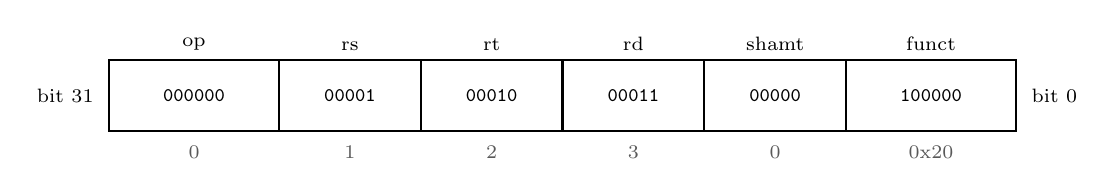
\begin{tikzpicture}[font=\small, x=0.36cm, y=0.9cm]
  \foreach \a/\b/\name/\val in {0/6/op/000000, 6/11/rs/00001, 11/16/rt/00010,
      16/21/rd/00011, 21/26/shamt/00000, 26/32/funct/100000} {
    \draw[thick] (\a,0) rectangle (\b,1);
    \node[font=\ttfamily\scriptsize] at ({(\a+\b)/2},0.5) {\val};
    \node[font=\scriptsize, above] at ({(\a+\b)/2},1) {\name};
  }
  \foreach \x/\v in {3/0, 8.5/1, 13.5/2, 18.5/3, 23.5/0, 29/{0x20}}
    \node[font=\scriptsize, gray!70!black] at (\x,-0.3) {\v};
  \node[font=\scriptsize, anchor=east] at (-0.2,0.5) {bit 31};
  \node[font=\scriptsize, anchor=west] at (32.2,0.5) {bit 0};
\end{tikzpicture}
\end{center}
Note that in assembly the destination comes first, but in the encoding
\code{rd} comes third.
\end{example}

\begin{example}
Encode \code{lw \$5, -8(\$29)}: op = 0x23, rs = 29, rt = 5, imm = $-8$
= \code{0xFFF8}. Bits: \code{100011 11101 00101 1111111111111000}
= \code{0x8FA5FFF8}.
\end{example}

\section*{Summary}
\begin{itemize}
  \item Five instructions: \code{add}, \code{sub}, \code{lw}, \code{sw},
    \code{beq}. Two R-format, three I-format.
  \item Memory addresses are base + signed byte offset; words are aligned.
  \item Branch offsets count instructions relative to $PC+4$.
  \item \code{beq \$0, \$0, k} acts as an unconditional branch.
  \item These five instructions drive the design of the single-cycle
    datapath later in the course.
\end{itemize}
